\part{Introduction}
\frame{\partpage}

\begin{frame}{Basics: Outline}
\small
  \tableofcontents[subsectionstyle=hide]%[pausesections]
  % You might wish to add the option [pausesections]
\end{frame}

\section{Who are we?}
\begin{frame}{UIS: Research and Institutional Services Division}
Your trainers for today will be:\\
\begin{itemize}
\item{Paul Sumption: Research Computing Technical Liaison}
\item{Arjen Tamerus: Research Software Engineer}
\end{itemize}
\end{frame}

\section{Training Accounts}
\begin{frame}{Basics: Training accounts}
\begin{itemize}
\item{\alert{For our practical exercise's we will use HPC training accounts.}}
\pause
\item{You will find two pieces of paper on your desk.}
\pause
\item{1: A terms and conditions form for you to sign.}
\pause
\item{2: Your training account details.}
\pause
\item{Your training account will only be valid for today.}
\end{itemize}
\end{frame}

\section{CSD 3 and Login node for today}
\begin{frame}{Basics: Login node}
\begin{itemize}
\item{\alert{For our practical exercise's we will use the login node login-gfx2.hpc.cam.ac.uk.}}
\pause
\item{Normally you would use login.hpc.cam.ac.uk hence using this in the examples in our slides.}
\pause
\item{We will be using nodes attached to Darwin}
\pause
\item{Some of the details in theses slides will change as we now have a new cluster CSD3 and Darwin is in the process of being decommissioned.}
\pause
\item{The main difference is the login node names and slightly different submit scripts as CSD 3 has more node types.}
\end{itemize}
\end{frame}

\section{Security}
\begin{frame}{Basics: Security}
\begin{itemize}
\item{\alert{Boring but very, very important${}\ldots$}}
\pause
\item{Cambridge IT is under constant attack by would-be intruders.}
\pause
\item{Your data and research career is threatened by intruders.}
\pause
\item{\alert{Cambridge systems} are high profile and popular targets.}
\pause
\item{\alert{Don't let intruders in.}}
\end{itemize}
\end{frame}

\begin{frame}{Basics: Security}
\begin{enumerate}
\item{\alert{Keep your password (or private key passphrase) safe.}}
\pause
\item{\alert{Always choose strong passwords.}}
\pause
\item{\alert{Your UIS password is used for multiple systems so keep it secure!}}
\pause
\item{Keep the software on your laptops/tablets/PCs up to date this includes home computers especially if you are using the VPN to connect in.}
\pause
\item{Don't share accounts (this is against the rules anyway).}
\end{enumerate}
\end{frame}

\section{Basics: Pre-requisites}
\begin{frame}{Pre-requisites}
\begin{itemize}
\item{A pre-requisite of this course:}
\pause
\item{Basic Unix/Linux command line experience}
\item{\url{https://www.training.cam.ac.uk/ucs/Course/ucs-unixintro1} Unix: Introduction to the Command Line Interface (Self-paced)}
\pause
\item{Shell scripting experience is desirable}
\item{\url{https://www.training.cam.ac.uk/ucs/Course/ucs-scriptsci} Unix: Simple Shell Scripting for Scientists}
\end{itemize}
\end{frame}

\section{Connecting}
\begin{frame}{Basics: Connecting}
\begin{itemize}
\item When connecting to the cluster will we use the SSH secure protocol only.\hfill\\
\item{We will use the Linux workstations during this course}
\item{Please check your workstation is booted into Ubuntu Linux, ask if you need help with this.}
\item{You are welcome to use your own laptop, however you may need to install some software in order to connect.}
\item{Later in this section of the slides we will cover the software you may need to install on your own computer.}
\end{itemize}
\end{frame}

\subsection{Connecting - SSH}
\begin{frame}{Basics: Connecting}
\begin{itemize}
\item SSH secure protocol only.\hfill\\
\visible<2->{\alert{Supports login, file transfer, remote desktop\ldots}}
\item<3-> HPCS allows access from registered IP addresses only.\hfill\\
\visible<4->{\alert{Almost all Cambridge University addresses already registered.}}
\visible<5->{\alert{Connection from home possible via the VPN service\hfill\\
\qquad http://www.ucs.cam.ac.uk/vpn}}\hfill\\
\visible<6->{\qquad\alert{or SSH tunnel through a departmental gateway.}}
\end{itemize}
\end{frame}

\subsection{Linux Clients}
\begin{frame}{Connecting: Linux Clients}
\begin{itemize}
\item {\color<2->{red}ssh}, scp, sftp, {\color<2->{red}rsync}\hfill\\
\alert{\small Installed (or installable), in Ubuntu we will use 'Terminal'.}
\item {X Windows, for using graphical applications remotely}
\alert{\small This is already installed on your desktop.}
\end{itemize}
\end{frame}

\subsection{Login}
\begin{frame}{Connecting: Login}
\begin{itemize}
\item From Linux/MacOSX/UNIX (or Cygwin):\hfill\\
\alert{ssh -Y \textbf{abc123}@login.hpc.cam.ac.uk}
\pause
\item From graphical clients:\hfill\\
Host: \alert{login.hpc.cam.ac.uk}\hfill\\
Username: \alert{\textbf{abc123}} (your UCAM account name)
\pause
\item login.hpc will map to a random login node\hfill\\
\alert{i.e. one of login-sand1, login-sand2,\,\ldots\,, login-sand8}\hfill\\
\uncover<4->{{\color{red}NB Not darwin.hpc (the head node).}}
\item<5->Non-registered addresses will fail with ``Connection refused''.
\item<6->Similarly for other systems (e.g.\ cardio-login.hpc, login-mrc-bsu.hpc,\ldots). 
\end{itemize}
\end{frame}

\subsection{First time login}
\begin{frame}{Connecting: First time login}
\begin{itemize}
\item{The first connection to a particular hostname produces the following:}
\begin{semiverbatim}\footnotesize
The authenticity of host 'login-sand2.hpc.cam.ac.uk (131.111.1.214)' can't be established.

RSA key fingerprint is

{\color<2->{red}0b:ef:59:90:fb:13:4a:c9:56:82:7b:cd:4b:2b:e1:3b}.

Are you sure you want to continue connecting (yes/no)? {\color<3->{red}yes}

Warning: Permanently added 'login-sand2.hpc.cam.ac.uk' (RSA) to the list of known hosts.
\end{semiverbatim}
\smallskip\item{\alert{One should always check the fingerprint before typing ``yes''.}}
\item{Graphical SSH clients \emph{should} ask a similar question.}
\item{Designed to detect fraudulent servers.}
\end{itemize}
\end{frame}

\begin{frame}[fragile]{Connecting: First time login}
\begin{itemize}
\item{You may be presented with any of the following fingerprints (depending on your client):}
\begin{semiverbatim}\footnotesize

MD5:0b:ef:59:90:fb:13:4a:c9:56:82:7b:cd:4b:2b:e1:3b
SHA256:sSkVfzpwjwiFvxLcdPoDpN8IsN3kt0ZSywhDhPKZPAg

MD5:34:9b:f2:d2:c6:b3:5c:63:99:b7:27:da:5b:c8:16:fe
SHA256:HsiY1Oe0M8tS6JwR76PeQQA/VB7r8675BzG5OYQ4h34

MD5:64:7c:7c:ff:05:9d:0e:dc:06:fe:f1:c2:10:37:7a:85
SHA256:wq9ljBfPa7lXXpQq+rk5JTBXLJO/kXjOc5A7rp4ENzA

\end{semiverbatim}
\end{itemize}
\end{frame}

\section{Basic practicals}
\begin{frame}{Basics: A practical example before some theory}
\begin{itemize}
\item{Some simple exercises will help us gauge your experience.}
\item{Exercise 1: Login with SSH.}
\item{Exercise 2: Navigating the command line.}
\item{Exercise 3: SFTP file transfer.}
\end{itemize}
\end{frame}

\subsection{Navigating the command line }
\begin{frame}{Navigating your terminal}
Useful commands for navigating your terminal.
\begin{itemize}
\item{\alert{\footnotesize cd \textless dirname \textgreater } - change into a directory }
\item{\alert{\footnotesize ls \textless dirname \textgreater } - list the contents of a directory}
\item{\alert{\footnotesize cd or cd \path{~}} - change into your home folder}
\item{\alert{\footnotesize cd .. } - change back one folder}
\item{\alert{\footnotesize man ls } - will bring up the manual page for the ls command}
\item{\alert{\footnotesize pwd } - print working directory}
\end{itemize}
\end{frame}

\subsection{Exercise 1: Navigating the command line}
\begin{frame}{Exercise 1: Navigating your terminal}
\begin{itemize}
\item{Start a terminal by double clicking on the terminal icon}
\item{Try the \alert{\footnotesize ls } and \alert{\footnotesize cd } commands in a terminal.}
\item{Look at the man page for the ls command}
\item{Close the terminal}
\end{itemize}
\end{frame}

\subsection{Exercise 2: Login}
\begin{frame}{Exercise 2: Login}
Using a Linux terminal you will login to the cluster with your HPC training account.
\begin{itemize}
\item{Start the terminal by double clicking on the terminal icon}
\item In your terminal enter:
\item{ssh -Y \textbf{abc123}@login.hpc.cam.ac.uk}\\
Replace abc123 with your training account username 
\item {Enter your password as supplied on the sheet}
\item{Leave this terminal open, you will need it for exercise 3!}
\end{itemize}
\end{frame}

%%%%
\subsection{Exercise 3: SFTP file transfer - pt1}
\begin{frame}{Exercise 3: Transfer some files}
You will need to transfer the exercise files to the cluster.
\begin{itemize}
\item{Open a second Linux terminal on your training computer.}
\item{Enter this command: cd \alert{\footnotesize \path{~\Course_material}}}
\item{Check the file 'exercises.tar.gz is in your directory listing}
\item{Hint: ls}
\end{itemize}
\end{frame}

\subsection{Exercise 3: SFTP file transfer - pt2}
\begin{frame}{Exercise 3: Transfer some files}
Transfer the exercises.tar.gz to your HPC home folder.
\begin{itemize}
\item \alert{\footnotesize sftp abc123@login.hpc.cam.ac.uk}\\
Change abc123 to your training account username
\item{The command: \alert{\footnotesize put exercises.tar.gz} will transfer the file from your local computer to the remote one}
\item{In terminal logged into the cluster type: ls}
\item{Use: tar -xvf exercise.tar  - to unzip the file}
\end{itemize}
\end{frame}

\subsection{File Transfer with rsync}
\begin{frame}{Connecting: File Transfer}
In exercise 3 we used sftp. Another tool to be familiar with is rsync especially when you want to transfer lots of directories and files.
\begin{itemize}
\item{rsync is a powerful tool and has many features.}
\item[$\ast$]You can rerun it to update or resume after interruption.
\item[$\ast$]All transfers are checksummed.
\end{itemize}
\end{frame}
%
\subsection{File Transfer with rsync: an example}
\begin{frame}{Connecting: File Transfer}
\begin{itemize}
\item From Linux/MacOSX/UNIX (or Cygwin):\hfill\\
\alert{\footnotesize rsync -av \textbf{old\_directory/} abc123@login.hpc.cam.ac.uk:scratch/new\_directory}\hfill\\
copies contents of old\_directory to $\tilde{}\text{/scratch/new\_directory}$.\hfill\\\smallskip
\pause
\alert{\footnotesize rsync -av \textbf{old\_directory} abc123@login.hpc.cam.ac.uk:scratch/new\_directory}\hfill\\
copies old\_directory (and contents) to $\tilde{}\text{/scratch/new\_directory/old\_directory}$.\hfill\\
\pause
\item[$\ast$]For transfers in the opposite direction, place the remote machine as the first argument.
\end{itemize}
\end{frame}
%
\section{Connecting from other clients}
\begin{frame}{Basics: Connecting from other clients}
\begin{itemize}
\item{When using your own computer you you may need to install some software in order to connect.}
\pause
\item{There are quite a few choices of software packages for this, we will just cover a few.}
\pause
\item{Our website https://www.hpc.cam.ac.uk/using-clusters/connecting covers this in more detail.}
\end{itemize}
\end{frame}

\subsection{MacOSX}
\begin{frame}{Connecting: MacOSX/UNIX Clients}
\begin{itemize}
\item {\color<2->{red}ssh}, scp, sftp, {\color<2->{red}rsync}\hfill\\
\alert{\small Installed (or installable) OS X has a native terminal package. This can be launched by clicking Apple \textgreater Go \textgreater Utilities and then clicking the Terminal icon.}
\item<3-> TurboVNC \alert{\small (for remote desktop, 3D optional)}\hfill\\
\alert{\small http://sourceforge.net/projects/turbovnc/files/}
\item<4-> On MacOSX, install \alert{XQuartz} to display remote graphical applications.\hfill\\
\alert{\small http://xquartz.macosforge.org/landing/}
\end{itemize}
\end{frame}

\subsection{Windows Users}
\begin{frame}{MobaXterm SSH (Windows)}
\begin{center}
\centerline{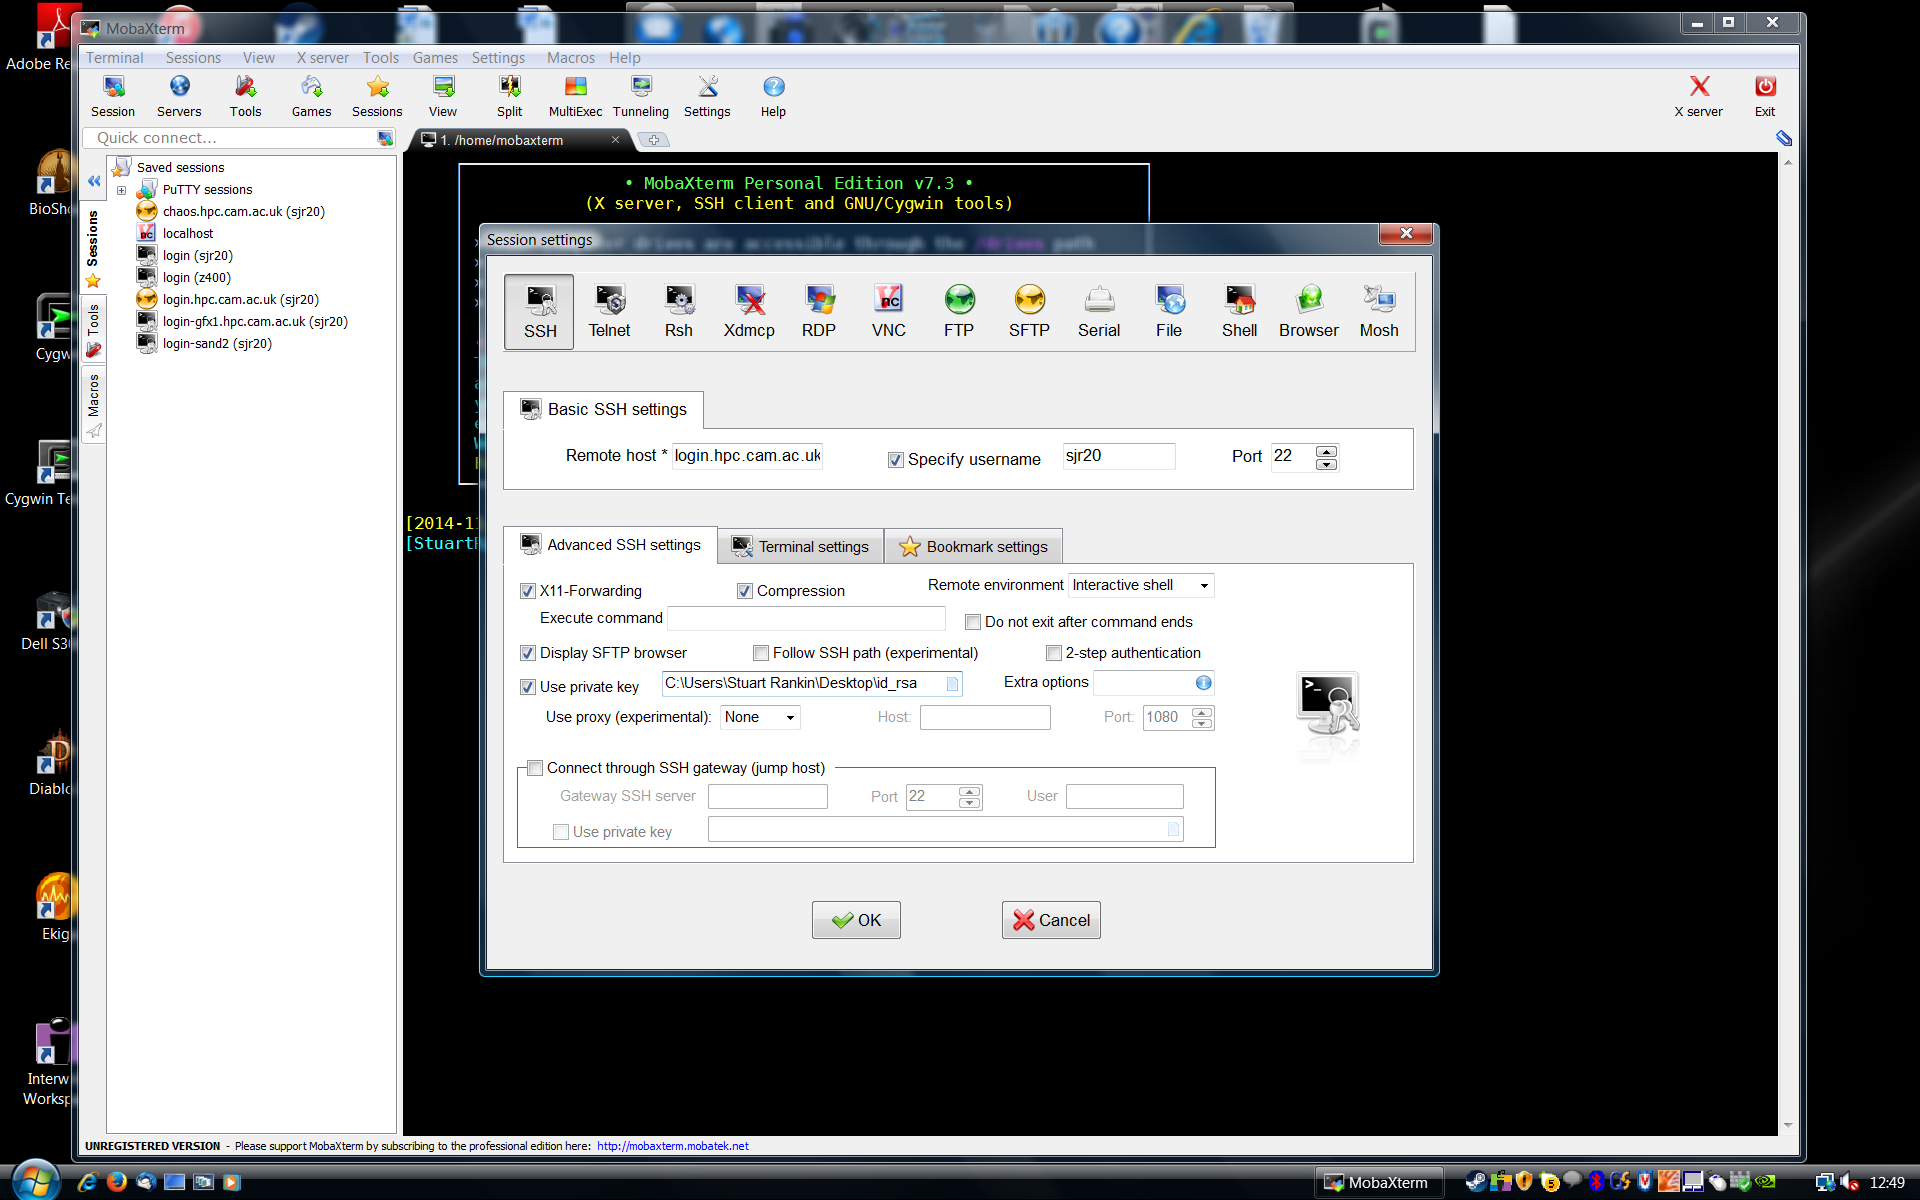
\includegraphics[height=0.8\textheight]{imgs/mobaxterm-SSH-settings2.png}}
\end{center}
\end{frame}

\begin{frame}{MobaXterm SSH (Windows)}
\begin{center}
\centerline{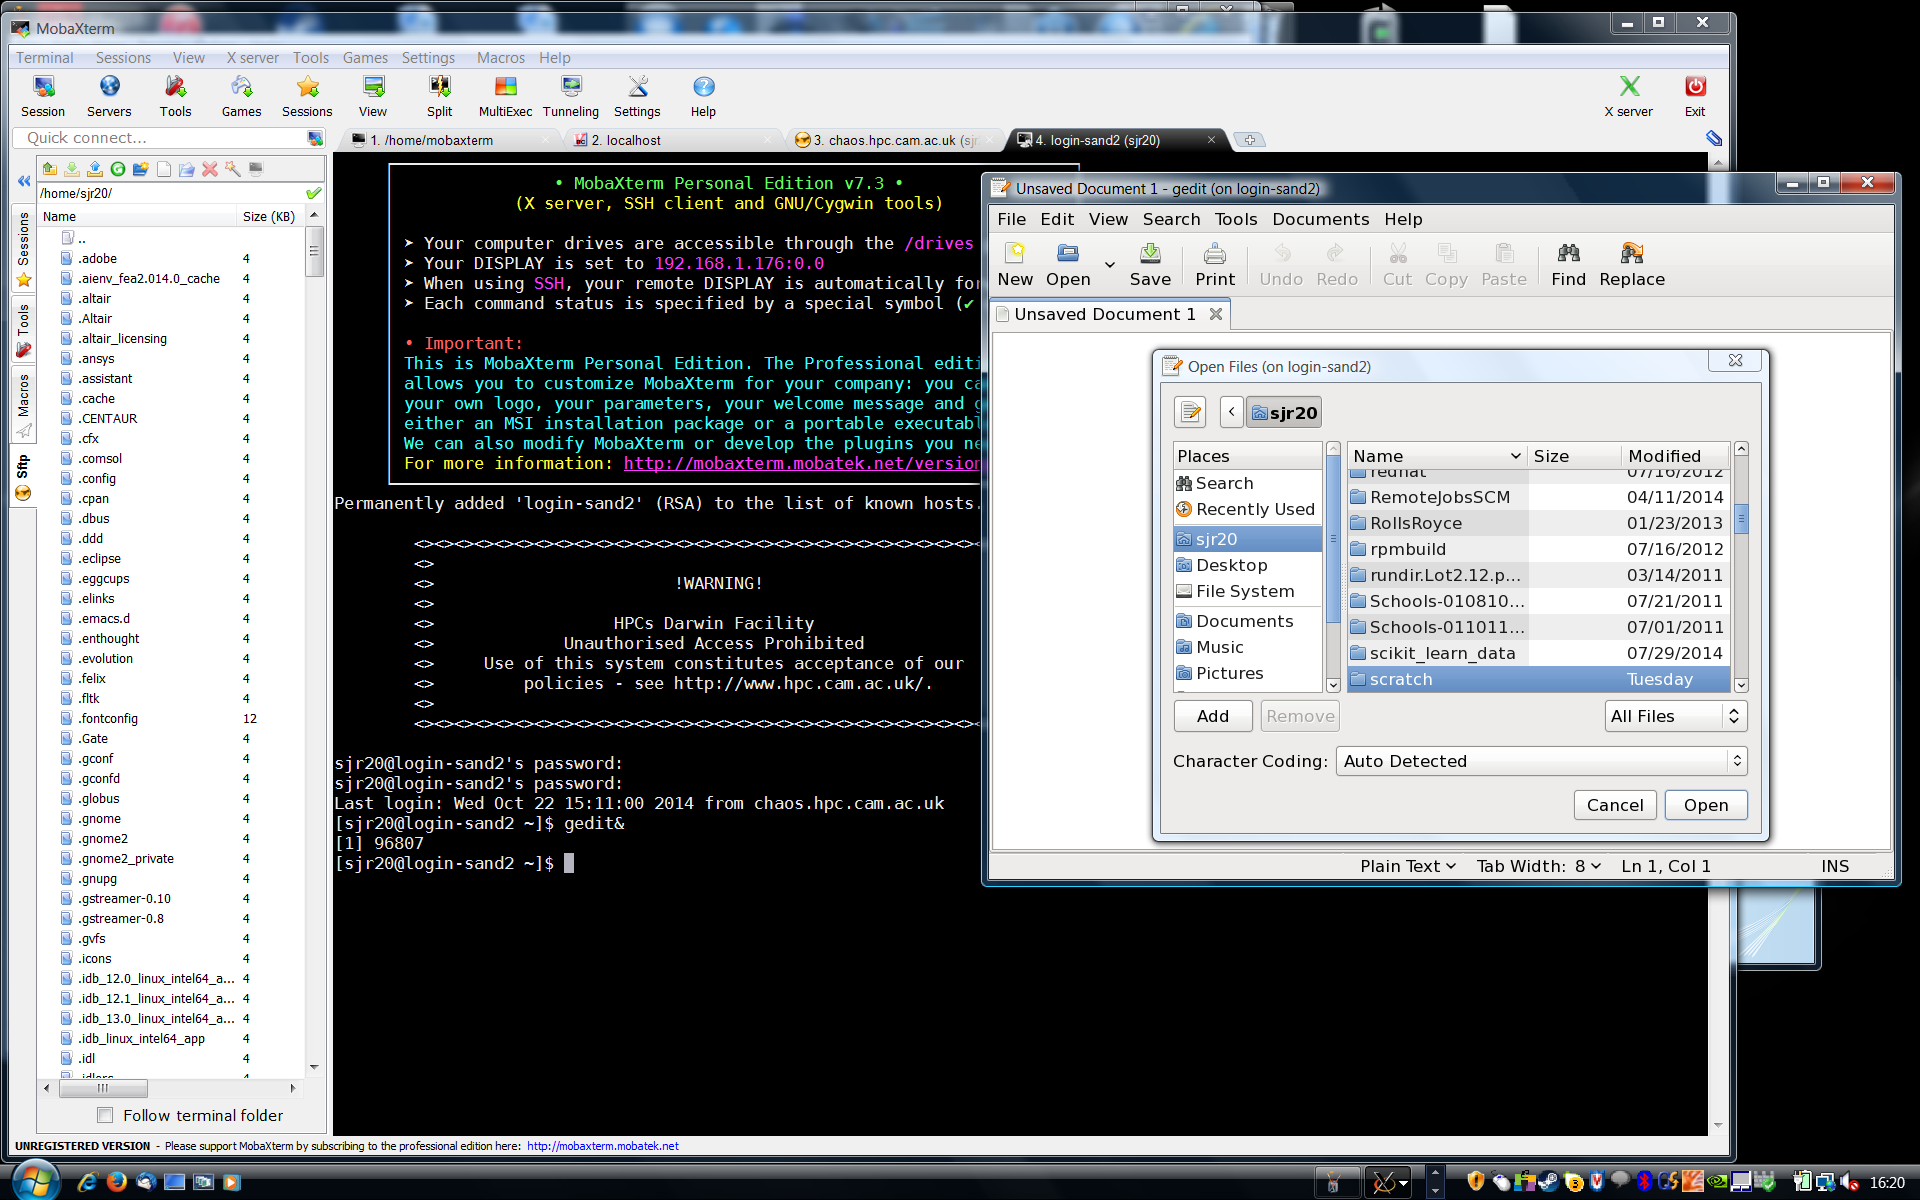
\includegraphics[height=0.8\textheight]{imgs/mobaxterm-SSH-session.png}}
\end{center}
\end{frame}